\section{Forsøg 1: Svingning af lod i luft i kort tid}\label{exp1: Forsog 1 - hele afsnittet}

\subsection{Forsøgsbeskrivelse}\label{exp1: Beskrivelse af experiment}
\subsubsection{Materialer}
\begin{wrapfigure}{r}{0.4\textwidth}
\centering
\opstillingEt{-1}%Se opstilling.sty i hovedmappen for definition. Ser bedst ud med udgangsposition i -1.

\caption{Skitse af forsøgsopsætning til forsøg 1. Den grå figur under loddet er en ultralydsensor.}
\label{fig:Forsogsopsaetning 1}
\end{wrapfigure} 

Disse materialer blev brugt til forsøget:
\begin{itemize}
	\setlength\itemsep{-1em}
	\item Lod - ca. $30g$
	\item Fjeder
	\item Kraftmåler
	\item Tavlelineal ($1$ meter)
	\item Stativ til opsætning
	\item Ultralydsensor
	\item Computer til opsamling af data
\end{itemize}

\subsubsection{Udførelsen}\label{exp1: Udforelse}



Før selve udførslen af forsøget bestemmer jeg en fjederkonstant for den fjeder, jeg arbejder med. 
Dette gøres ved at måle samhørende værdier af udstrækning af fjederen, og hvor stor en kraft den trækker med. 

I dette forsøg har jeg opsat et lod i en fjeder, som set på figur \ref{fig:Forsogsopsaetning 1}.
Derefter har jeg sat loddet i svingninger og målt loddets position med ultralydsensoren i en periode på $10$ sekunder. 
Jeg gentog dette forsøg 10 gange. 


\subsection{Hypotese}\label{exp1: Hypotese}
Da dette forsøg forløber over forholdsvist kort tid, forventer jeg, at man kan betragte denne bevægelse, som om den ikke er dæmpet, da dæmpningsledet vil være forholdsvis småt og vil virke i kort tid. 
Dermed forventes differentialligningen 
$$m\cdot x'' = -k \cdot x$$
at være opfyldt, jvf. afsnit \ref{teori: Opstilling ligning uden dampning}.
Dette kan omskrives til $m\cdot x'' + k\cdot x=0$, hvilket vi ser er en andenordens lineær homogen differentialligning. 
Vi kan derfor bestemme en karakterligning som $mr^2 + k = 0 \Rightarrow r^2 + \frac{k}{m} = 0$ og dermed får vi $r = \frac{\pm \sqrt{-4\frac{k}{m}}}{2}=\pm\sqrt{\frac{k}{m}}i$.
Dermed skal vi have fat i den løsning af differentialligningen, hvor løsningerne til karakterligningen er komplekse. 
Vi får da, at løsningen skal være på formen (se afsnit \ref{teori: Komplekse losninger i karakterligningen}):

$$y(x) = e^{ax}A\sin(bx+\phi) \text{ hvor rødderne i karakterligningen er } r = a \pm bi$$

Vi ser dog her, at rødderne i vores karakterligning ikke har nogen realdel, og dermed får vi at $e^{ax}=e^{0x}=1$.
Da $b=\sqrt{\frac{k}{m}}$ forventer vi derfor, at bevægelsen vil kunne beskrives som 
\begin{equation}
x(t)=A\sin (\frac{k}{m}t+\phi)
\label{eq: exp1 hypotese}
\end{equation}

hvor $\phi$ er en eller anden konstant. 

\begin{wrapfigure}{r}{0.4\textwidth}
\centering
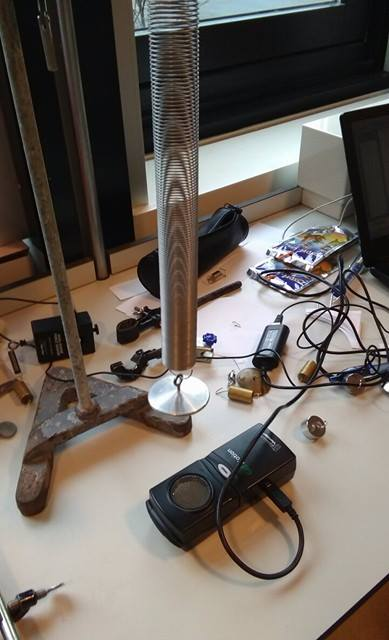
\includegraphics[scale=0.4]{Figurer/Opstilling}
\caption{Billede af forsøgopstilling der blev brugt i forsøg 1 og 2.}
\end{wrapfigure}

\subsection{Data}\label{exp1: Data}


Data til dette forsøg er vedlagt som bilag i filen ''Forsøg 1 - Data.pdf''.
Denne fil indeholder alt rådata opsamlet af ultralydsensoren i de 10 forsøg (OBS. filen er $130$ sider lang, da der er blevet opsamlet $40$ målinger i sekundet). 
Forsøg nummer 10 er placeret først, grundet måden mit dataopsamlingsprogram fungerer på.

\subsubsection{Fjederkonstant}\label{exp1: Fjederkonstant}
Ydermere er der vedlagt en fil ved navn ''Forsøg 1 og 2 fjederkonstant - Data.pdf''.
Denne fil indeholder data til bestemmelse af fjederkonstanten. 

\subsubsection{Masse af fjeder og lod}\label{exp1: Masse af fjeder og lod}
Jeg har målt massen af lodet og af fjederen i forbindelse med forsøget. 
Disse to er nedskrevet i tabel \ref{tabel: Masser forsog 1}.
\pagebreak
\begin{table}[h]
\centering
\begin{tabular}{|c|c|}
\hline 
 & Masse ($g$) \\ 
\hline 
Fjeder & $77.09$ \\ 
\hline 
Lod & $32.45$ \\ 
\hline 
\end{tabular} 
\caption{Relevante masser til forsøg 1.}
\label{tabel: Masser forsog 1}
\end{table}

\subsection{Databehandling}\label{exp1: databehandling afsnit}
\subsubsection{Fjederkonstant}\label{databehandling: tyk fjeder fjederkonstant}
For at bestemme fjederkonstanten for fjederen, der bliver brugt til forsøget, har jeg taget de sammenhørende værdier af fjederkraft og udstrækning og plottet dem med kraft som afhængig og udstrækning som uafhængig variabel. 
Derefter har jeg lavet en best-fit lineær sammenhæng. 
Denne har en forholdsvist lav RMSE på $0.044N$, og derfor virker dataen pålidelig. 
Vi må da have fjederkonstanten som hældningen på dette plot, i dette tilfælde $3.6\frac{N}{m}$.

Den tilhørende graf samt best-fit plot kan ses i bilaget "Forsøg 1 - grafer.pdf". 
 

\subsubsection{Best-fit kurver}\label{exp1: Best-fit kurver}
For at tjekke hvor godt hypotesen holder, har jeg fået min computer til at lave en best-fit kurve udfra funktionen $x(t)=A\sin (\sqrt{\frac{k}{m}}+\phi) + s_0$.
Det tilføjede $s_0$ for enden skyldes, at loddet har hængt en afstand over ultralydsensoren, som der skal justeres for. 

I tabel \ref{tabel: bestfitkurver forsog 1} kan ses værdier for $A, \sqrt{\frac{k}{m}}, \phi ,s_0$ og så den gennemsnitlige afvigelse målt i meter (RMSE).


\begin{table}[h]
\centering
\begin{tabular}{|l|c|c|c|c|c|}
\hline
\textbf{}          & \textbf{A}($m$) & \textbf{$\sqrt{\frac{k}{m}}$}($s^{-1}$) & \textbf{$\phi$} & \textbf{$s_0$}($m$) & \textbf{RMSE }($m$) \\ \hline
\textbf{Forsøg 10} & 0,08854    & 7,73                          & 584,8           & 0,2929         & 0,003136      \\ \hline
\textbf{Forsøg 1}  & 0,04319    & 7,632                         & 6,99            & 0,2984         & 0,001839      \\ \hline
\textbf{Forsøg 2}  & 0,06744    & 7,669                         & 20,9            & 0,2963         & 0,001766      \\ \hline
\textbf{Forsøg 3}  & 0,07559    & 7,692                         & 38,58           & 0,2948         & 0,002061      \\ \hline
\textbf{Forsøg 4}  & 0,081      & 7,707                         & -1,786          & 0,2933         & 0,003476      \\ \hline
\textbf{Forsøg 5}  & 0,08944    & 7,734                         & -1,145          & 0,2936         & 0,004427      \\ \hline
\textbf{Forsøg 6}  & 0,08174    & 7,709                         & 3,467           & 0,294          & 0,00381       \\ \hline
\textbf{Forsøg 7}  & 0,06552    & 7,663                         & 818,2           & 0,2954         & 0,001818      \\ \hline
\textbf{Forsøg 8}  & 0,05712    & 7,648                         & 9,939           & 0,2965         & 0,001589      \\ \hline
\textbf{Forsøg 9}  & 0,04544    & 7,633                         & 9,7             & 0,297          & 0,001462      \\ \hline
\end{tabular}

\caption{De forskellige værdier på best-fit kurver. De tilhørende grafer til dataen samt best-fit-plot er vedlagt som bilag i filen ''Forsøg 1 - grafer.pdf''}
\label{tabel: bestfitkurver forsog 1}
\end{table}

\subsubsection{Sammenligning af værdier af $\sqrt{\frac{k}{m}}$}\label{exp1: teoretisk bestemmelse af sqrt k over m}
For at tjekke om konstanter tager de forventede værdier, vil jeg sammenligne værdierne for $\sqrt{\frac{k}{m}}$ fundet ved best-fit-kurven og ved måling på fjeder og lod.

Værdierne fra best-fit-kurven, der kan ses i tabel \ref{tabel: bestfitkurver forsog 1}, er meget ens, og jeg vil derfor bare bruge et gennemsnit af dem. 
Dette gennemsnit bliver da ca. $7.68s^{-1}$.

Massen af loddet og fjederkonstanten har jeg begge bestemt individuelt. 
Fjederkonstanten kender jeg som $3.6\frac{N}{m}$ (se tidligere i dette afsnit). 
Massen er lidt mindre ligetil. 
Vi kender godt nok massen af loddet fra tabel \ref{tabel: Masser forsog 1}. 
Der er dog det problem, at det ikke kun er loddet, der svinger i bevægelsen, men også en del af fjederen. 
I teorien er det ca. $\frac{1}{3}$ af fjederens masse der skal regnes med i bevægelsen\refFysA{300}.
Vi kan derfor lave en masse $m=m_{lod}+\frac{1}{3}\cdot m_{fjeder}=32.45g+\frac{77.09g}{3}=58.15g$. 
Dermed kan vi bestemme en værdi for $\sqrt{\frac{k}{m}}$ som:
$$\sqrt{\frac{k}{m}}=\sqrt{\frac{3.6\frac{N}{m}}{58.15g}}=\sqrt{0.062\frac{\frac{N}{m}}{g}}=\sqrt{0.062\frac{1000\frac{g\cdot m}{s^2\cdot m}}{g}}=\sqrt{62s^{-2}}=7.87s^{-1}$$

Værdien fået ved best-fit ser ud til at stemme rimelig godt overens med den målte, da de har en forholdsvist lille differens på $0.19s^{-1}$. 



\subsubsection{Vurdering af data}\label{exp1: Vurdering af data}

\begin{itemize}

\item Værdierne af $\sqrt{\frac{k}{m}}$ ligger meget tæt på hinanden. 
Dette stemmer godt overens med teorien, da denne værdi ikke bør være afhængig af, hvor meget energi, der bliver tilført systemet til at starte med, men kun lodets masse og fjederens fjederkonstant. 
Da forsøget er lavet med samme fjeder og samme lod, må man forvente samme værdi, hvilket også er det vi observerer, da der kun er en forskel på $7.734s^{-1}-7.632s^{-1}=0.102s^{-1}$ på den største og mindste værdi, hvilket er relativt lidt i forhold til de ca. $7.5$ tallene ligger på.



\item Afvigelserne er meget lave. 
Den gennemsnitlige afvigelse ligger imellem $0.3136cm$ og $0.4427cm$ i forhold til amplituderne på helt op til $8.944cm$. 
Dette må anses som forholdsvis små afvigelser i forhold til hele bevægelsen.



\item Værdien $\sqrt{\frac{k}{m}}$ i de fundne best-fit kurver er meget tæt på den værdi, man kan finde ved at veje lodet og bestemme fjederkonstanten.



\item Der er meget stor variation af værdien af $\phi$.
Dette er dog ikke noget problem, da denne størrelse for det første bare er afhængig af, hvornår i bevægelsen målingen er startet.
Derudover har den så store udsving fordi sinusfunktionen er periodisk med en periode på $2\pi$.
Vi kunne derfor have fjernet eller tilføjet $2\pi$ et heltalligt antal gange uden at have påvirket grafen det mindste. 
Derfor er forskellene i værdier ikke bekymrende. 


\end{itemize}

\subsection{Konklusion}
Dette forsøg stemmer godt med teorien. 
Der er høje forklaringsgrader ved brug af best-fit kurver, og de værdier som kommer ud med de forskellige konstanter, passer godt overens med vores teori.
Det forekommer derfor sandsynligt, at bevægelsen tilnærmelsesvist opfylder hypotesen og dermed differentialligningen \ref{eq: exp1 hypotese}.

